

% Команда \sun для отрисовки точечного источника света (солнышка)
\newcommand{\sun}{\tikz[baseline=-0.5ex]{
  \draw[thick, black, fill=white] (0,0) circle (2pt);
  \foreach \angle in {0,45,90,135,180,225,270,315} {
    \draw[black, thin] (\angle:3.2pt) -- (\angle:5.2pt);
  }
}}

% === ЗАДАЧА 1 ===
% Тег: #ОПТИКА #ЛИНЗЫ #ПОСТРОЕНИЕ_ИЗОБРАЖЕНИЙ #КИМ_13
\begin{taskbasic}[code={\label{task:optics_lens_point_source_v1}}]
Какая из точек (1, 2, 3, 4, 5 или 6), показанных на рисунке, является изображением точечного источника света $S$, полученным в тонкой собирающей линзе с фокусным расстоянием $F$?

\nopagebreak\smallskip
\begin{center}
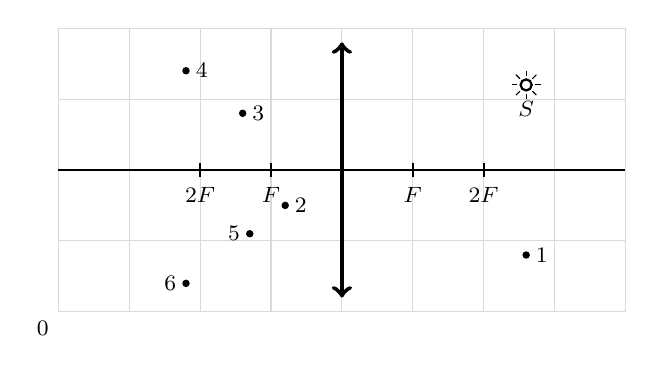
\begin{tikzpicture}[scale=0.9, every node/.style={font=\footnotesize}]
    \draw[xstep=1, ystep=1, gray!30, thin] (-4,-2) grid (4,2);
    
    % Главная оптическая ось
    \draw[thick, black] (-4,0) -- (4,0);
    
    % Собирающая линза
    \draw[ultra thick, black, <->] (0,-1.8) -- (0,1.8);
    
    % Фокусы
    \draw[thick, black] (-1,0.1) -- (-1,-0.1) node[below] {$F$};
    \draw[thick, black] (-2,0.1) -- (-2,-0.1) node[below] {$2F$};
    \draw[thick, black] (1,0.1) -- (1,-0.1) node[below] {$F$};
    \draw[thick, black] (2,0.1) -- (2,-0.1) node[below] {$2F$};
    
    % Источник S (справа вверху, за 2F)
    \node at (2.6,1.2) {$\sun$};
    \node[below] at (2.6,1.1) {$S$};
    
    % Точки изображений
    \fill[black] (2.6,-1.2) circle (1.5pt) node[right] {1};
    \fill[black] (-0.8,-0.5) circle (1.5pt) node[right] {2};
    \fill[black] (-1.4,0.8) circle (1.5pt) node[right] {3};
    \fill[black] (-2.2,1.4) circle (1.5pt) node[right] {4};
    \fill[black] (-1.3,-0.9) circle (1.5pt) node[left] {5};
    \fill[black] (-2.2,-1.6) circle (1.5pt) node[left] {6};
    
    \node[below left] at (-4,-2) {0};
\end{tikzpicture}
\end{center}

\kim{13}
\end{taskbasic}
\answer{5}

% === ЗАДАЧА 2 ===
% Тег: #ОПТИКА #ЛИНЗЫ #ПОСТРОЕНИЕ_ИЗОБРАЖЕНИЙ #КИМ_13
\begin{taskbasic}[code={\label{task:optics_lens_point_source_v2}}]
Какая из точек (1, 2, 3, 4, 5 или 6), показанных на рисунке, является изображением точечного источника света $S$, полученным в тонкой собирающей линзе с фокусным расстоянием $F$?

\nopagebreak\smallskip
\begin{center}
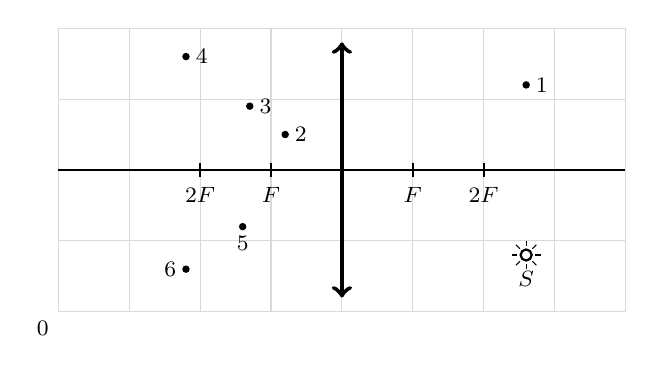
\begin{tikzpicture}[scale=0.9, every node/.style={font=\footnotesize}]
    \draw[xstep=1, ystep=1, gray!30, thin] (-4,-2) grid (4,2);
    
    \draw[thick, black] (-4,0) -- (4,0);
    \draw[ultra thick, black, <->] (0,-1.8) -- (0,1.8);
    
    \draw[thick, black] (-1,0.1) -- (-1,-0.1) node[below] {$F$};
    \draw[thick, black] (-2,0.1) -- (-2,-0.1) node[below] {$2F$};
    \draw[thick, black] (1,0.1) -- (1,-0.1) node[below] {$F$};
    \draw[thick, black] (2,0.1) -- (2,-0.1) node[below] {$2F$};
    
    % Источник S (справа внизу, за 2F)
    \node at (2.6,-1.2) {$\sun$};
    \node[below] at (2.6,-1.3) {$S$};
    
    % Точки
    \fill[black] (2.6,1.2) circle (1.5pt) node[right] {1};
    \fill[black] (-0.8,0.5) circle (1.5pt) node[right] {2};
    \fill[black] (-1.3,0.9) circle (1.5pt) node[right] {3};
    \fill[black] (-2.2,1.6) circle (1.5pt) node[right] {4};
    \fill[black] (-1.4,-0.8) circle (1.5pt) node[below] {5};
    \fill[black] (-2.2,-1.4) circle (1.5pt) node[left] {6};
    
    \node[below left] at (-4,-2) {0};
\end{tikzpicture}
\end{center}

\kim{13}
\end{taskbasic}
\answer{3}

% === ЗАДАЧА 3 ===
% Тег: #ОПТИКА #ЛИНЗЫ #ПОСТРОЕНИЕ_ИЗОБРАЖЕНИЙ #КИМ_13
\begin{taskbasic}[code={\label{task:optics_lens_point_source_2f}}]
Какая из точек (1, 2, 3 или 4) является изображением точечного источника света $S$ в собирающей тонкой линзе с фокусным расстоянием $F$ (см. рисунок)?

\nopagebreak\smallskip
\begin{center}
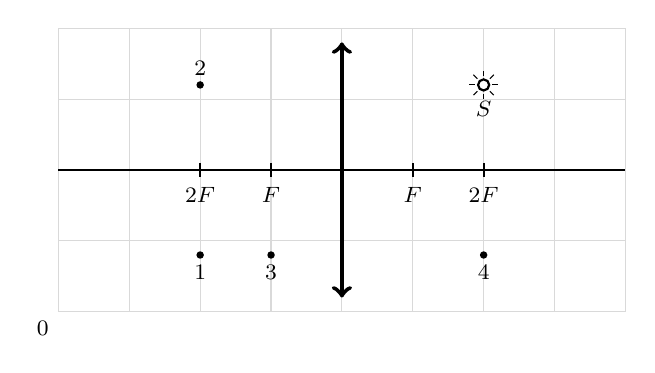
\begin{tikzpicture}[scale=0.9, every node/.style={font=\footnotesize}]
    \draw[xstep=1, ystep=1, gray!30, thin] (-4,-2) grid (4,2);
    
    \draw[thick, black] (-4,0) -- (4,0);
    \draw[ultra thick, black, <->] (0,-1.8) -- (0,1.8);
    
    \draw[thick, black] (-1,0.1) -- (-1,-0.1) node[below] {$F$};
    \draw[thick, black] (-2,0.1) -- (-2,-0.1) node[below] {$2F$};
    \draw[thick, black] (1,0.1) -- (1,-0.1) node[below] {$F$};
    \draw[thick, black] (2,0.1) -- (2,-0.1) node[below] {$2F$};
    
    % Источник S (в 2F)
    \node at (2.0,1.2) {$\sun$};
    \node[below] at (2.0,1.1) {$S$};
    
    % Точки
    \fill[black] (-2.0,-1.2) circle (1.5pt) node[below] {1};
    \fill[black] (-2.0,1.2) circle (1.5pt) node[above] {2};
    \fill[black] (-1.0,-1.2) circle (1.5pt) node[below] {3};
    \fill[black] (2.0,-1.2) circle (1.5pt) node[below] {4};
    
    \node[below left] at (-4,-2) {0};
\end{tikzpicture}
\end{center}

\kim{13}
\end{taskbasic}
\answer{1}

% === ЗАДАЧА 4 ===
% Тег: #ОПТИКА #ЛИНЗЫ #РАСЧЕТНАЯ_ЗАДАЧА #КИМ_25
\begin{taskbasic}[code={\label{task:optics_lens_two_sources_dptr}}]
Два точечных источника света находятся на главной оптической оси тонкой собирающей линзы с оптической силой $4\text{ дптр}$ на некотором расстоянии $L$ друг от друга. Линза находится между ними. Расстояние от линзы до одного из источников $x = 20\text{ см}$. Изображения обоих источников получились в одной точке. Найдите расстояние $L$. Постройте на отдельных рисунках изображения двух источников в линзе, указав ход лучей. Ответ выразите в метрах (м).

\kim{25}
\end{taskbasic}
\answer{1,25}

% === ЗАДАЧА 5 ===
% Тег: #ОПТИКА #ЛИНЗЫ #ПОСТРОЕНИЕ_ИЗОБРАЖЕНИЙ #КИМ_13
\begin{taskbasic}[code={\label{task:optics_lens_point_source_2f_bottom}}]
Какая из точек (1, 2, 3 или 4) является изображением точечного источника света $S$ в собирающей тонкой линзе с фокусным расстоянием $F$ (см. рисунок)?

\nopagebreak\smallskip
\begin{center}
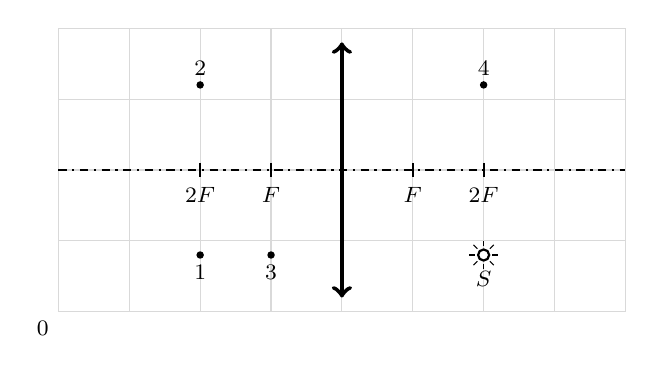
\begin{tikzpicture}[scale=0.9, every node/.style={font=\footnotesize}]
    \draw[xstep=1, ystep=1, gray!30, thin] (-4,-2) grid (4,2);
    
    \draw[thick, black, dash dot] (-4,0) -- (4,0);
    \draw[ultra thick, black, <->] (0,-1.8) -- (0,1.8);
    
    \draw[thick, black] (-1,0.1) -- (-1,-0.1) node[below] {$F$};
    \draw[thick, black] (-2,0.1) -- (-2,-0.1) node[below] {$2F$};
    \draw[thick, black] (1,0.1) -- (1,-0.1) node[below] {$F$};
    \draw[thick, black] (2,0.1) -- (2,-0.1) node[below] {$2F$};
    
    % Источник S
    \node at (2.0,-1.2) {$\sun$};
    \node[below] at (2.0,-1.3) {$S$};
    
    % Точки
    \fill[black] (-2.0,-1.2) circle (1.5pt) node[below] {1};
    \fill[black] (-2.0,1.2) circle (1.5pt) node[above] {2};
    \fill[black] (-1.0,-1.2) circle (1.5pt) node[below] {3};
    \fill[black] (2.0,1.2) circle (1.5pt) node[above] {4};
    
    \node[below left] at (-4,-2) {0};
\end{tikzpicture}
\end{center}

\kim{13}
\end{taskbasic}
\answer{2}

% === ЗАДАЧА 6 ===
% Тег: #ОПТИКА #ЛИНЗЫ #РАСЧЕТНАЯ_ЗАДАЧА #КИМ_25
\begin{taskbasic}[code={\label{task:optics_lens_two_sources_l1m}}]
Два точечных источника света находятся на главной оптической оси тонкой собирающей линзы на расстоянии $L = 1\text{ м}$ друг от друга. Линза находится между ними. Расстояние от линзы до одного из источников $x = 20\text{ см}$. Изображения обоих источников получились в одной точке. Найдите оптическую силу линзы. Постройте на отдельных рисунках изображения двух источников в линзе, указав ход лучей. Ответ выразите в диоптриях (дптр).

\kim{25}
\end{taskbasic}
\answer{6,25}

% === ЗАДАЧА 7 ===
% Тег: #ОПТИКА #ЛИНЗЫ #ПОСТРОЕНИЕ_ИЗОБРАЖЕНИЙ #КИМ_13
\begin{taskbasic}[code={\label{task:optics_lens_optical_axis_ray}}]
Какая из точек (1, 2, 3 или 4), показанных на рисунке, служит изображением точки $S$ (см. рисунок), создаваемым тонкой собирающей линзой с фокусным расстоянием $F$?

\nopagebreak\smallskip
\begin{center}
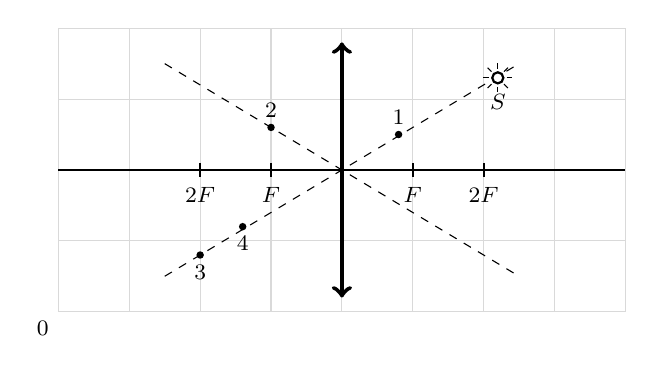
\begin{tikzpicture}[scale=0.9, every node/.style={font=\footnotesize}]
    \draw[xstep=1, ystep=1, gray!30, thin] (-4,-2) grid (4,2);
    
    \draw[thick, black] (-4,0) -- (4,0);
    \draw[ultra thick, black, <->] (0,-1.8) -- (0,1.8);
    \draw[dashed, black] (-2.5,1.5) -- (2.5,-1.5);
    \draw[dashed, black] (-2.5,-1.5) -- (2.5,1.5);
    
    \draw[thick, black] (-1,0.1) -- (-1,-0.1) node[below] {$F$};
    \draw[thick, black] (-2,0.1) -- (-2,-0.1) node[below] {$2F$};
    \draw[thick, black] (1,0.1) -- (1,-0.1) node[below] {$F$};
    \draw[thick, black] (2,0.1) -- (2,-0.1) node[below] {$2F$};
    
    \node at (2.2,1.3) {$\sun$};
    \node[below] at (2.2,1.2) {$S$};
    
    \fill[black] (0.8,0.5) circle (1.5pt) node[above] {1};
    \fill[black] (-1.0,0.6) circle (1.5pt) node[above] {2};
    \fill[black] (-2.0,-1.2) circle (1.5pt) node[below] {3};
    \fill[black] (-1.4,-0.8) circle (1.5pt) node[below] {4};
    
    \node[below left] at (-4,-2) {0};
\end{tikzpicture}
\end{center}

\kim{13}
\end{taskbasic}
\answer{3}

% === ЗАДАЧА 8 ===
% Тег: #ОПТИКА #ЛИНЗЫ #ПОСТРОЕНИЕ_ИЗОБРАЖЕНИЙ #КИМ_13
\begin{taskbasic}[code={\label{task:optics_lens_optical_axis_ray_bottom}}]
Какая из точек (1, 2, 3 или 4), показанных на рисунке, служит изображением точки $S$ (см. рисунок), создаваемым тонкой собирающей линзой с фокусным расстоянием $F$?

\nopagebreak\smallskip
\begin{center}
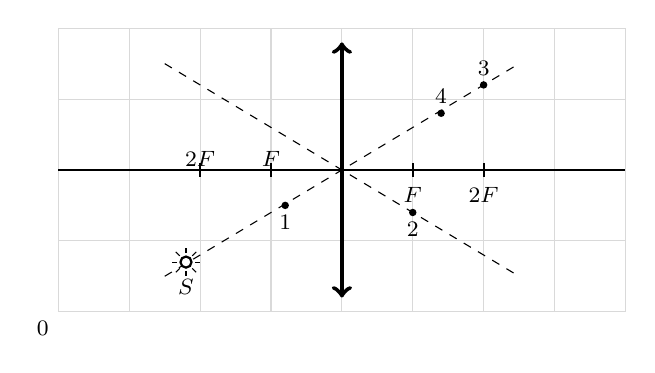
\begin{tikzpicture}[scale=0.9, every node/.style={font=\footnotesize}]
    \draw[xstep=1, ystep=1, gray!30, thin] (-4,-2) grid (4,2);
    
    \draw[thick, black] (-4,0) -- (4,0);
    \draw[ultra thick, black, <->] (0,-1.8) -- (0,1.8);
    \draw[dashed, black] (-2.5,1.5) -- (2.5,-1.5);
    \draw[dashed, black] (-2.5,-1.5) -- (2.5,1.5);
    
    \draw[thick, black] (-1,0.1) -- (-1,-0.1) node[above] {$F$};
    \draw[thick, black] (-2,0.1) -- (-2,-0.1) node[above] {$2F$};
    \draw[thick, black] (1,0.1) -- (1,-0.1) node[below] {$F$};
    \draw[thick, black] (2,0.1) -- (2,-0.1) node[below] {$2F$};
    
    \node at (-2.2,-1.3) {$\sun$};
    \node[below] at (-2.2,-1.4) {$S$};
    
    \fill[black] (-0.8,-0.5) circle (1.5pt) node[below] {1};
    \fill[black] (1.0,-0.6) circle (1.5pt) node[below] {2};
    \fill[black] (2.0,1.2) circle (1.5pt) node[above] {3};
    \fill[black] (1.4,0.8) circle (1.5pt) node[above] {4};
    
    \node[below left] at (-4,-2) {0};
\end{tikzpicture}
\end{center}

\kim{13}
\end{taskbasic}
\answer{3}

% === ЗАДАЧА 9 ===
% Тег: #ОПТИКА #ЛИНЗЫ #ПОСТРОЕНИЕ_ИЗОБРАЖЕНИЙ #КИМ_13
\begin{taskbasic}[code={\label{task:optics_lens_inside_focus}}]
Какая из точек (1, 2, 3 или 4) является изображением точечного источника $S$, создаваемым тонкой собирающей линзой с фокусным расстоянием $F$ (см. рисунок)?

\nopagebreak\smallskip
\begin{center}
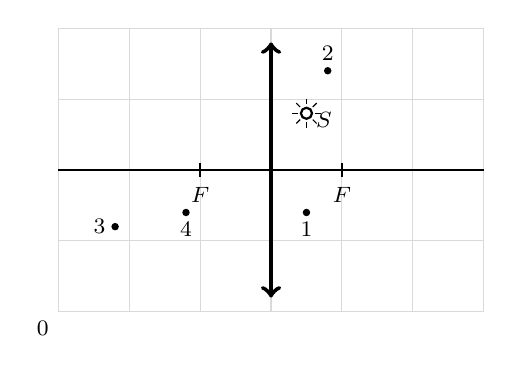
\begin{tikzpicture}[scale=0.9, every node/.style={font=\footnotesize}]
    \draw[xstep=1, ystep=1, gray!30, thin] (-3,-2) grid (3,2);
    
    \draw[thick, black] (-3,0) -- (3,0);
    \draw[ultra thick, black, <->] (0,-1.8) -- (0,1.8);
    
    \draw[thick, black] (-1,0.1) -- (-1,-0.1) node[below] {$F$};
    \draw[thick, black] (1,0.1) -- (1,-0.1) node[below] {$F$};
    
    \node at (0.5,0.8) {\textbf{$\sun$}};
    \node[right] at (0.5,0.7) {$S$};
    
    \fill[black] (0.5,-0.6) circle (1.5pt) node[below] {1};
    \fill[black] (0.8,1.4) circle (1.5pt) node[above] {2};
    \fill[black] (-2.2,-0.8) circle (1.5pt) node[left] {3};
    \fill[black] (-1.2,-0.6) circle (1.5pt) node[below] {4};
    
    \node[below left] at (-3,-2) {0};
\end{tikzpicture}
\end{center}

\kim{13}
\end{taskbasic}
\answer{3}

% === ЗАДАЧА 10 ===
% Тег: #ОПТИКА #ЛИНЗЫ #ПОСТРОЕНИЕ_ИЗОБРАЖЕНИЙ #КИМ_13
\begin{taskbasic}[code={\label{task:optics_lens_inside_focus_right}}]
Какая из точек (1, 2, 3 или 4) является изображением точечного источника $S$, создаваемым тонкой собирающей линзой с фокусным расстоянием $F$ (см. рисунок)?

\nopagebreak\smallskip
\begin{center}
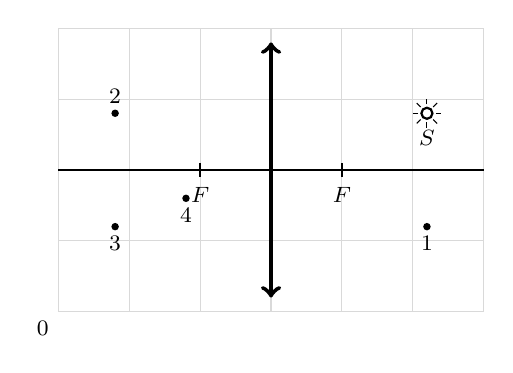
\begin{tikzpicture}[scale=0.9, every node/.style={font=\footnotesize}]
    \draw[xstep=1, ystep=1, gray!30, thin] (-3,-2) grid (3,2);
    
    \draw[thick, black] (-3,0) -- (3,0);
    \draw[ultra thick, black, <->] (0,-1.8) -- (0,1.8);
    
    \draw[thick, black] (-1,0.1) -- (-1,-0.1) node[below] {$F$};
    \draw[thick, black] (1,0.1) -- (1,-0.1) node[below] {$F$};
    
    \node at (2.2,0.8) {\textbf{$\sun$}};
    \node[below] at (2.2,0.7) {$S$};
    
    \fill[black] (2.2,-0.8) circle (1.5pt) node[below] {1};
    \fill[black] (-2.2,0.8) circle (1.5pt) node[above] {2};
    \fill[black] (-2.2,-0.8) circle (1.5pt) node[below] {3};
    \fill[black] (-1.2,-0.4) circle (1.5pt) node[below] {4};
    
    \node[below left] at (-3,-2) {0};
\end{tikzpicture}
\end{center}

\kim{13}
\end{taskbasic}
\answer{3}

% === ЗАДАЧА 1 ===
% Тег: #ОПТИКА #ЛИНЗЫ #ПОСТРОЕНИЕ_ИЗОБРАЖЕНИЙ #КИМ_13
\begin{taskbasic}[code={\label{task:optics_lens_item_to_image_v1}}]
Какому из предметов 1--4 соответствует изображение $AB$ в тонкой собирающей линзе с фокусным расстоянием $F$?

\nopagebreak\smallskip
\begin{center}
\begin{tikzpicture}[scale=0.9, every node/.style={font=\footnotesize}]
    \draw[xstep=1, ystep=1, gray!30, thin] (-4,-2) grid (4,2);
    
    % Главная оптическая ось
    \draw[thick, black] (-4,0) -- (4,0);
    \draw[ultra thick, black, <->] (0,-1.8) -- (0,1.8);
    
    % Побочные оси
    \draw[dashed, black] (-3,1.5) -- (3,-1.5);
    \draw[dashed, black] (-3,-1.5) -- (3,1.5);
    
    % Фокусы
    \draw[thick, black] (-1,0.1) -- (-1,-0.1) node[below] {$F$};
    \draw[thick, black] (-2,0.1) -- (-2,-0.1) node[below] {$2F$};
    \draw[thick, black] (1,0.1) -- (1,-0.1) node[below] {$F$};
    \draw[thick, black] (2,0.1) -- (2,-0.1) node[below] {$2F$};
    
    % Изображение AB
    \draw[-{Stealth[scale=0.8]}, line width=1.5pt, black] (1.3,0) -- (1.3,0.65) node[pos=0, below] {$A$} node[pos=1, above] {$B$};
    
    % Предметы 1-4
    \draw[-{Stealth[scale=0.8]}, thick, black] (-1.3,0) -- (-1.3,0.65) node[right] {1};
    \draw[-{Stealth[scale=0.8]}, thick, black] (-0.8,0) -- (-0.8,-0.4) node[right] {2};
    \draw[-{Stealth[scale=0.8]}, thick, black] (-2.6,0) -- (-2.6,-1.3) node[left] {3};
    \draw[-{Stealth[scale=0.8]}, thick, black] (1.3,0) -- (1.3,-0.65) node[right] {4};
    
    \node[below left] at (-4,-2) {0};
\end{tikzpicture}
\end{center}

\kim{13}
\end{taskbasic}
\answer{1}

% === ЗАДАЧА 2 ===
% Тег: #ОПТИКА #ЛИНЗЫ #ПОСТРОЕНИЕ_ИЗОБРАЖЕНИЙ #КИМ_13
\begin{taskbasic}[code={\label{task:optics_lens_item_to_image_v2}}]
Какому из предметов 1--4 соответствует изображение $AB$ в тонкой собирающей линзе с фокусным расстоянием $F$?

\nopagebreak\smallskip
\begin{center}
\begin{tikzpicture}[scale=0.9, every node/.style={font=\footnotesize}]
    \draw[xstep=1, ystep=1, gray!30, thin] (-4,-2) grid (4,2);
    
    \draw[thick, black] (-4,0) -- (4,0);
    \draw[ultra thick, black, <->] (0,-1.8) -- (0,1.8);
    
    \draw[dashed, black] (-3,1.5) -- (3,-1.5);
    \draw[dashed, black] (-3,-1.5) -- (3,1.5);
    
    \draw[thick, black] (-1,0.1) -- (-1,-0.1) node[below] {$F$};
    \draw[thick, black] (-2,0.1) -- (-2,-0.1) node[below] {$2F$};
    \draw[thick, black] (1,0.1) -- (1,-0.1) node[below] {$F$};
    \draw[thick, black] (2,0.1) -- (2,-0.1) node[below] {$2F$};
    
    % Изображение AB
    \draw[-{Stealth[scale=0.8]}, line width=1.5pt, black] (2.6,0) -- (2.6,1.3) node[pos=0, below left] {$A$} node[pos=1, above] {$B$};
    
    % Предметы
    \draw[-{Stealth[scale=0.8]}, thick, black] (-1.3,0) -- (-1.3,0.65) node[right] {1};
    \draw[-{Stealth[scale=0.8]}, thick, black] (-1.3,0) -- (-1.3,-0.65) node[left] {2};
    \draw[-{Stealth[scale=0.8]}, thick, black] (-2.6,0) -- (-2.6,-1.3) node[right] {3};
    \draw[-{Stealth[scale=0.8]}, thick, black] (1.3,0) -- (1.3,-0.65) node[right] {4};
    
    \node[below left] at (-4,-2) {0};
\end{tikzpicture}
\end{center}

\kim{13}
\end{taskbasic}
\answer{3}

% === ЗАДАЧА 3 ===
% Тег: #ОПТИКА #ЛИНЗЫ #РАСЧЕТНАЯ_ЗАДАЧА #КИМ_25
\begin{taskbasic}[code={\label{task:optics_lens_screen_movement}}]
Линза, фокусное расстояние которой $30\text{ см}$, даёт на экране резкое изображение предмета с пятикратным увеличением. Экран пододвинули к линзе вдоль её главной оптической оси. Затем при неизменном положении линзы передвинули предмет на $3\text{ см}$ так, чтобы изображение снова стало резким. На какое расстояние сдвинули экран относительно его первоначального положения? Сделайте рисунок построения изображений в линзе с указанием хода лучей. Ответ выразите в сантиметрах (см).

\kim{25}
\end{taskbasic}
\answer{45}

% === ЗАДАЧА 4 ===
% Тег: #ОПТИКА #ЛИНЗЫ #СВЕТОВОЕ_ПЯТНО #КИМ_25
\begin{taskbasic}[code={\label{task:optics_lens_light_spot_diameter}}]
На двойном фокусном расстоянии от собирающей линзы с оптической силой $5\text{ дптр}$ на её главной оптической оси расположен точечный источник света. Линза вставлена в непрозрачную оправу радиусом $8\text{ см}$. Каков диаметр светлого пятна на экране, расположенном на расстоянии $60\text{ см}$ от линзы? Сделайте рисунок с указанием хода лучей. Ответ выразите в сантиметрах (см).

\kim{25}
\end{taskbasic}
\answer{8}

% === ЗАДАЧА 5 ===
% Тег: #ОПТИКА #ЛИНЗЫ #ГЕОМЕТРИЯ_ИЗОБРАЖЕНИЯ #КИМ_25
\begin{taskbasic}[code={\label{task:optics_lens_triangle_image_area}}]
Прямоугольный треугольник с катетами $c = 2\text{ см}$ и $h = 4\text{ см}$ расположен перед собирающей линзой с фокусным расстоянием $F = 10\text{ см}$, как показано на рисунке. Постройте изображение треугольника, даваемое линзой. Чему равна площадь этого изображения? Ответ выразите в квадратных сантиметрах ($\text{см}^2$).

\nopagebreak\smallskip
\begin{center}
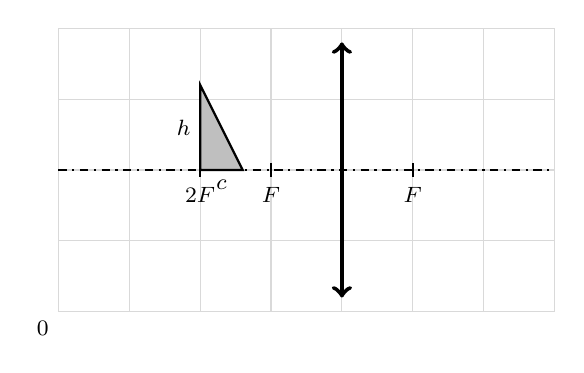
\begin{tikzpicture}[scale=0.9, every node/.style={font=\footnotesize}]
    \draw[xstep=1, ystep=1, gray!30, thin] (-4,-2) grid (3,2);
    
    \draw[thick, black, dash dot] (-4,0) -- (3,0);
    \draw[ultra thick, black, <->] (0,-1.8) -- (0,1.8);
    
    \draw[thick, black] (-1,0.1) -- (-1,-0.1) node[below] {$F$};
    \draw[thick, black] (-2,0.1) -- (-2,-0.1) node[below] {$2F$};
    \draw[thick, black] (1,0.1) -- (1,-0.1) node[below] {$F$};
    
    % Треугольник (катеты c и h)
    \draw[thick, black, fill=gray!50] (-2,0) -- (-2,1.2) -- (-1.4,0) -- cycle;
    \node[left] at (-2,0.6) {$h$};
    \node[below] at (-1.7,0) {$c$};
    
    \node[below left] at (-4,-2) {0};
\end{tikzpicture}
\end{center}

\kim{25}
\end{taskbasic}
\answer{11,25}